\documentclass[12pt]{beamer}

\usetheme{Warsaw}
\useoutertheme{split}
\useinnertheme{circles}
\usecolortheme{crane}

\usepackage{polski}
\usepackage[utf8]{inputenc}
\usepackage[english,polish]{babel}

\usepackage{xcolor}
\definecolor{default_color}{RGB}{0,0,0}
\colorlet{dcolor}{default_color}
\setbeamercolor{title}{fg=dcolor}
\setbeamercolor{titlelike}{fg=dcolor}
\setbeamercolor{frametitle}{fg=dcolor}

\usepackage{listings}
\lstdefinestyle{customcpp}{
  belowcaptionskip=1\baselineskip,
  breaklines=true,
  frame=L,
  xleftmargin=\parindent,
  language=C++,
  showstringspaces=false,
  basicstyle=\fontsize{9pt}{9}\ttfamily,
  keywordstyle=\bfseries\color{green!40!black},
  commentstyle=\itshape\color{purple!40!black},
  stringstyle=\color{orange},
}
\lstset{
	backgroundcolor=\color{white},
	language=C++,
	style=customcpp,
	tabsize=2
}


\usepackage{enumerate}
\setbeamertemplate{enumerate item}{$\textcolor{dcolor}{\insertenumlabel.}$}
\setbeamertemplate{enumerate subitem}{$\textcolor{dcolor}{\insertenumlabel.\insertsubenumlabel.}$}
\setbeamertemplate{enumerate subsubitem}{$\textcolor{dcolor}{\insertenumlabel.\insertsubenumlabel.\insertsubsubenumlabel.}$}

\setbeamertemplate{itemize item}{$\textcolor{dcolor}-$}
\setbeamertemplate{itemize subitem}{$\textcolor{dcolor}\bullet$}
\setbeamertemplate{itemize subsubitem}{$\textcolor{dcolor}\triangleright$}

\usepackage{tikz}
\usebackgroundtemplate{
	\tikz[overlay,remember picture]\node[opacity=0.4]at (current page.center){
		% source: https://upload.wikimedia.org/wikipedia/commons/thumb/1/18/ISO_C%2B%2B_Logo.svg/1822px-ISO_C%2B%2B_Logo.svg.png
		
\includegraphics[width=4cm]{cpp_logo.png}
	};
}

\title{Omówienie stanu prac pracy magisterskiej}
\subtitle{Przegląd bibliotek do serializacji w języku C++}
\author[inż. Krzysztof Mochocki]{inż. Krzysztof Mochocki}
\date{}


\begin{document}

	\begin{frame}
		\maketitle
	\end{frame}

	\begin{frame}
		\frametitle{Wstęp}
		\begin{enumerate}
			\item Geneza
			\item Problematyka serializacji
			\item Dostępne rozwiązania
			\item Schemat działania
			\item Badanie
		\end{enumerate}
	\end{frame}

	\begin{frame}[fragile]
		\frametitle{Dostępne rozwiązania}

		Manualna serializacja wspomagana przez zewnętrzną bibliotekę (np.: Microsoft Cpp Rest SDK)\newline

		\begin{lstlisting}[frame=single]
std::string serialize_my_class(const MyClass& obj)
{
	lib::json json{};
	json["field_0"] = lib::json::to_json_bool(obj.field_0);
	json["field_1"] = lib::json::to_json_int(obj.field_1);
	json["field_2"] = lib::json::to_json_string(obj.field_2);
	if(obj.field_3 == std::nullptr)
		json["field_3"] = lib::json::null();
	else
		json["field_3"] = lib::json::iterable_to_json(*obj.field_3, my_function_for_each_item);

	return json.to_string();
}
		\end{lstlisting}

	\end{frame}

	\begin{frame}[fragile]
		\frametitle{Dostępne rozwiązania}

		Automatyczna serializacja z manualną refleksją pól \newline(np.: Boost)

		\begin{lstlisting}[frame=single]
// MyClass.h
struct MyClass
{
	using svec_t = std::shared_ptr<std::vector<OtherClass>>;
	bool field_0;
	int field_1;
	std::string field_2;
	svec_t field_3;
};

// macro
LIB_REFLECT( my::namespace::MyClass, (field_0)(field_1)(field_2)(field_3) );

// main.cpp
std::string serialize_my_class(const MyClass& obj)
{
	return lib::json::to_string(obj);
}
		\end{lstlisting}

	\end{frame}

	\begin{frame}[fragile]
		\frametitle{Proponowane rozwiązanie}

		Automatyczna serializacja z automatyczną refleksją pól\newline

		\begin{lstlisting}[frame=single]
struct MyClassImpl
{
	using svec_t = std::shared_ptr<std::vector<OtherClass>>;
	lib::ffield<bool>											field_0;
	lib::field<&MyClassImpl::field_0, int>				field_1;
	lib::field<&MyClassImpl::field_1, std::string> 	field_2;
	lib::field<&MyClassImpl::field_2, svec_t>			field_3;
};
using MyClass = lib::pack<&MyClassImpl::field_3>;

std::string serialize_my_class(const MyClass& obj)
{
	return lib::json::to_string(obj);
}
		\end{lstlisting}

	\end{frame}

	\begin{frame}
		\frametitle{Schemat działania}

		\begin{figure}[ht!]
			\centering
			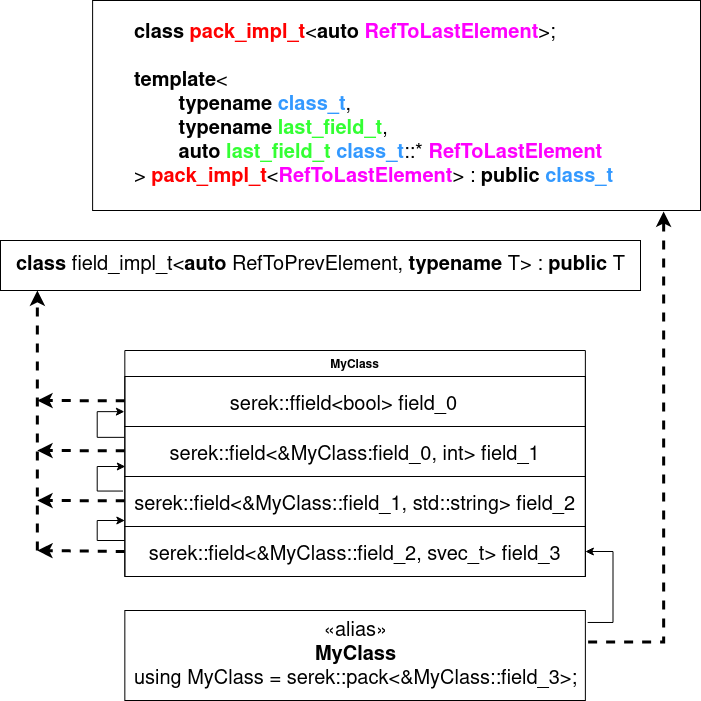
\includegraphics[width=0.75\framewidth, keepaspectratio=true]{./basic_concept_of_serek_UML.png}
			\caption{Diagram UML z konceptem stojącym za biblioteką serek}
		\end{figure}

	\end{frame}

	\begin{frame}
		\frametitle{Badanie}

			\begin{itemize}
				\item Narzut kodu do obsługi warstwy transportowej
				\begin{itemize}
					\item Ile czasu zajmuje serializacja
					\item Ile czasu zajmuje deserializacja
				\end{itemize}
				\item Łatwość w wytwarzaniu oprogramowania
				\begin{itemize}
					\item Ile \% kodu implementacji klasy zajmuje jej warstwa transportowa
					\item Całkowita ilość kodu wymagana do napisania hierarchii klas
					\item Objętość komunikatu o błędzie
				\end{itemize}
			\end{itemize}

	\end{frame}

	\begin{frame}
		\frametitle{Koniec}

		\centering\Huge Dziękuje za uwagę!

	\end{frame}

\end{document}
